\documentclass[a4paper,12pt]{report}
\usepackage[utf8]{inputenc}
\usepackage[francais]{babel}
\usepackage[T1]{fontenc}
\usepackage{graphicx}
\usepackage{listingsutf8}
\usepackage[colorlinks,urlcolor=blue]{hyperref} %hyperlinks
\usepackage[nottoc,notlot,notlof]{tocbibind} %To bind the table of contents to the bibligoraphy
\usepackage{../../../packages/tikz-uml} %UML elements

\begin{document}
%----------------------------------------------------------------------------------------
%   TITLE PAGE
%----------------------------------------------------------------------------------------
\begin{titlepage}
\newcommand{\HRule}{\rule{\linewidth}{0.5mm}} % Defines a new command for the horizontal lines
\center
%----------------------------------------------------------------------------------------
%   LOGOS SECTION
%----------------------------------------------------------------------------------------

\includegraphics[scale=0.5]{images/umLogo.png} % Université de Montpellier Logo
\hspace{\fill}

\includegraphics[scale=0.25]{images/fdsLogo.jpg} % Faculté de Sciences Logo
%----------------------------------------------------------------------------------------
%   HEADING SECTIONS
%----------------------------------------------------------------------------------------
\textsc{\LARGE M1 Informatique AIGLE}\\[1cm]
\textsc{\Large \textbf{HMIN122M}}\\[0.25cm]
\textsc{\large Mini-Projet : entrepôts de données}\\[0.8cm]
%----------------------------------------------------------------------------------------
%   TITLE SECTION
%----------------------------------------------------------------------------------------
\HRule \\[0.4cm]
{ \huge \bfseries Rapport}\\[0.4cm]
\HRule \\[0.8cm]
%----------------------------------------------------------------------------------------
%   AUTHORS SECTION
%----------------------------------------------------------------------------------------
\begin{minipage}{\textwidth}
\centering \huge
Bachar \textsc{Rima}\\ % Student
Joseph \textsc{Saba}\\ % Student
Tasnim \textsc{Shaqura Muhammad}\\ % Student
Jérémy \textsc{Bourgin} % Student
\end{minipage} \\[0.8cm]
%----------------------------------------------------------------------------------------
%   DATE SECTION
%----------------------------------------------------------------------------------------
{\large \today}\\[1cm]
\hspace{\fill}
\vfill % Fill the rest of the page with whitespace
\end{titlepage}

\pagestyle{plain}

{
  \hypersetup{linkcolor=black}
  \tableofcontents
}

\newpage

\chapter{Introduction}
\section{Problématiques}
Dans le cadre du mini-projet du module \textbf{HMIN122M}, nous avons décidé de modéliser un entrepôt de données pour le réseau de transport publique de Montpellier, \textit{tam-voyages}. Pour ce faire, nous avons proposé des \textit{data marts} formant le \textit{data warehouse} et permettant de réaliser des requêtes analytiques sur un ensemble important de données. Cette modélisation permettra ainsi de mettre en \oe{}uvre un outil d'analyse permettant de bien répondre aux problématiques suivantes :
\begin{enumerate}
  \item Comment \textit{tam-voyages} pourront-ils profiter de la fréquentation de leurs véhicules en se basant sur la circulation du réseau\footnote{en particulier en examinant les lignes de tramway et les bus} pour améliorer la qualité de leur service (e.g. \textit{nombre de véhicules à envoyer sur une ligne pendant une certaine période de la journée})?
  \item Comment \textit{tam-voyages} pourront-ils suivre l'évolution et la maintenance de leurs matériaux de manière à réduire les dépenses qui y sont associées ?
\end{enumerate}

Ces problématiques seront ainsi adressées en analyzant les actions et opérations effectuées par \textit{tam-voyages}, notamment en choisissant celles qui paraissent les plus pertinentes et les plus importantes en termes de données intégrées et flexibilité des critères d'analyse.

\section{Actions et opérations}
Les actions/opérations effectuées par \textit{tam-voyages} considérées :
\begin{itemize}
  \item Les voyages.
  \item La maintenance de véhicules.
  \item Les ventes de tickets et les abonnements.
  \item Les amendes.
\end{itemize}

Les actions considérées, par ordre d'importance:
\begin{enumerate}
  \item \og voyages \fg.
  \item \og ventes \fg.
  \item \og maintenance \fg.
  \item \og amendes \fg.
\end{enumerate}

Les actions les plus pertinentes à analyser vis-à-vis les problématiques avancées sont \og voyages \fg et \og maintenance \fg qu'on traitera de la manière suivante :
\begin{description}
  \item [voyages :] modèle en étoile détaillé.
  \item [maintenance :] modèle en étoile \textit{moins} détaillé, en particulier le modèle intitulé "\textit{periodic snapshot}".
\end{description}

\section{Exemples de requêtes analytiques possibles}
\begin{enumerate}
  \item exemples de requêtes analytiques pour l'action \og voyages \fg :
  \begin{itemize}
    \item \texttt{le nombre de voyageurs par bus, utilisant des tickets pour le mois de juillet.}
    \item \texttt{le prix moyen par voyage pendant les vacances de noël de 2018.} :
    \item \texttt{le nombre de voyageurs abonnés par ligne pour chaque voyage pour les deux derniers mois.}
    \item \texttt{l'arrêt le plus fréquenté par toutes les lignes de circulation.}
  \end{itemize}
  \item exemples de requêtes analytiques pour l'action \og maintenance \fg :
  \begin{itemize}
    \item \texttt{le nombre de bus maintenus pour le mois de septembre 2018.}
    \item \texttt{les X méchaniciens les plus expérimentés convoqués pour la maintenance des bus l'année précédente.}
    \item \texttt{les X premières véhicules nécessitant le plus de maintenance pour les 6 dernier mois.}
  \end{itemize}
  \item exemples de requêtes analytiques pour l'action \og ventes \fg :
  \begin{itemize}
    \item \texttt{le nombre d'abonnés ayant plus que 26 ans pour le mois d'août 2018.}
    \item \texttt{le nombre d'abonnés par date de naissance pour l'année 2018.}
    \item \texttt{les types d'abonnement les plus fréquents pour l'année 2018.}
  \end{itemize}
  \item exemples de requêtes analytiques pour l'action \og amendes \fg :
  \begin{itemize}
    \item \texttt{les lignes qui ont générées le plus d'amendes pour les deux derniers mois.}
    \item \texttt{les lignes les plus contrôllées de la semaine dernière.}
    \item \texttt{le nombre des abonnés qui ont reçu des amendes par ligne, l'avant-midi.}
    \item \texttt{la somme total d'amendes rapportée par type de voyageur par ligne pour le dernier mois.}
  \end{itemize}
\end{enumerate}

\chapter{Modélisation}
\begin{figure}[!ht]
  \centering
  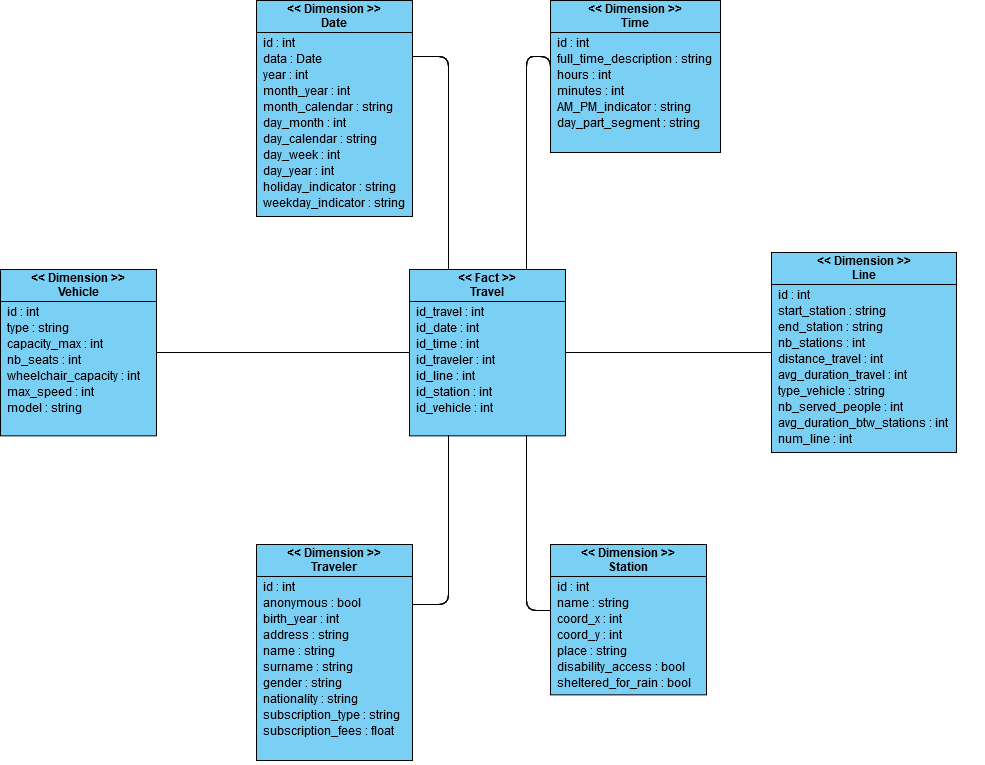
\includegraphics[scale=0.4]{images/voyages_datamart.png}
  \caption{modèle en étoile de l'action \og voyages \fg}
\end{figure}

\newpage

La table des voyages n'admet aucune mesure; on se contentera d'utiliser les informations fournies par les dimensions qui suffiront largement pour analyser la fréquentation des différentes lignes et véhicules correspondant.

\begin{figure}[!ht]
  \centering
  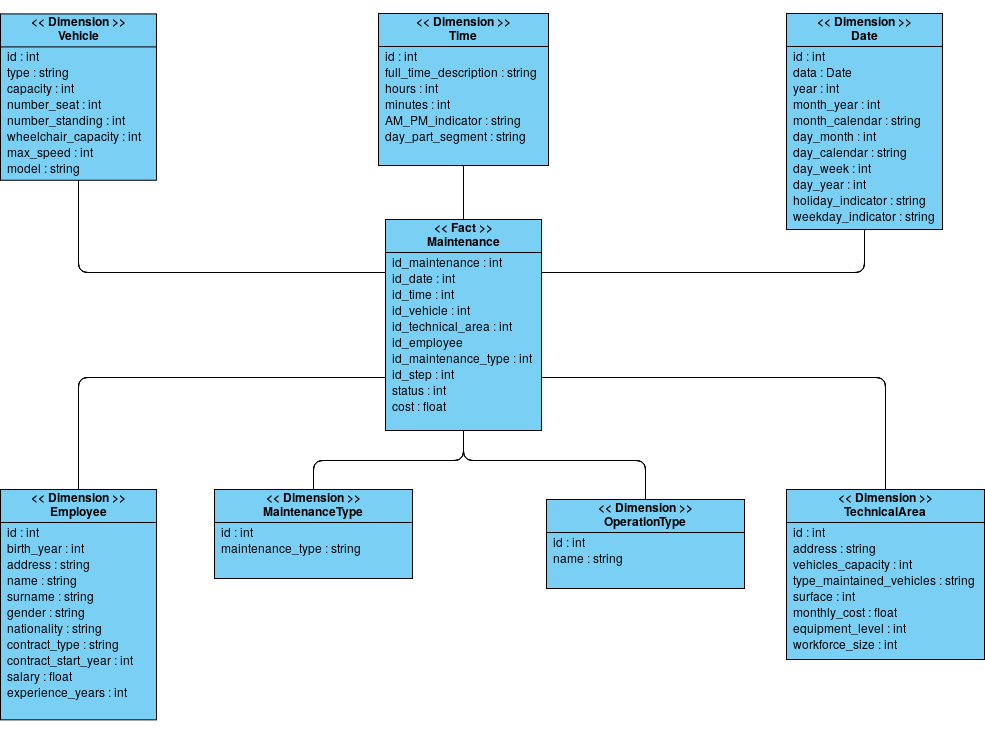
\includegraphics[scale=0.4]{images/maintenance_datamart.png}
  \caption{modèle en étoile de l'action \og maintenance \fg}
\end{figure}

Les mesures de la table des maintenances sont :
\begin{itemize}
  \item \texttt{cost} : mesure additive désignant le coût de maintenance d'un véhicule pour une transaction donnée
\end{itemize}

\newpage

\begin{figure}[!ht]
  \centering
  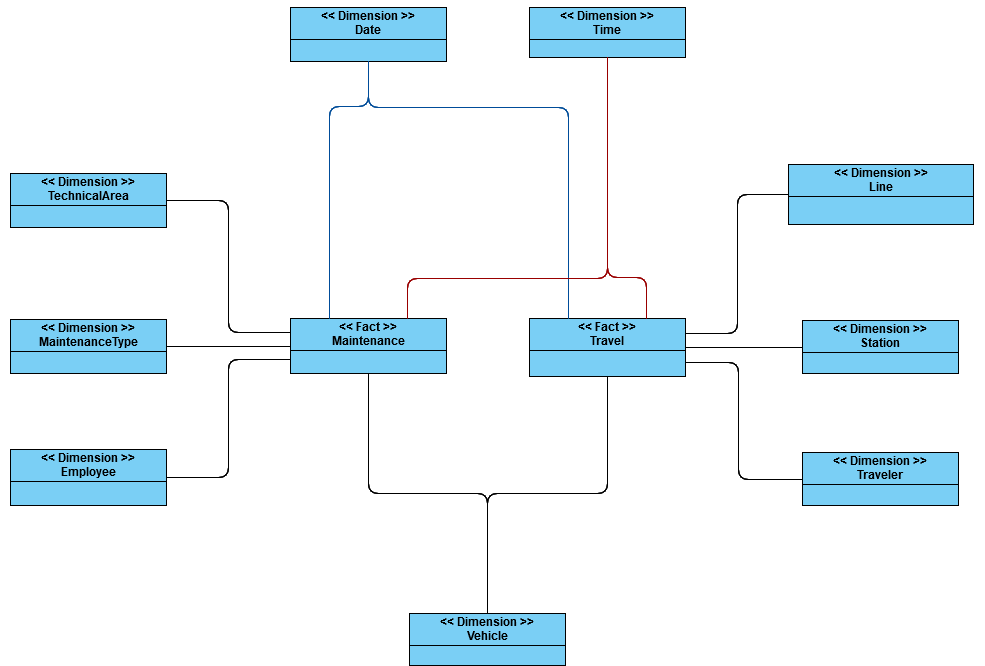
\includegraphics[scale=0.4]{images/data_warehouse.png}
  \caption{le \textit{data warehouse} résultant}
\end{figure}

\subsubsection{Remarques}
\begin{itemize}
  \item l'attribut \textbf{id\_travel} de la table \texttt{Travel} est la clé primaire utilisée pour identifier un voyage (\textit{dimension dégénérée}).
  \item l'attribut \textbf{nb\_served\_people} de la table \texttt{Line} désigne le nombre de passagers désservis par la ligne.
  \item l'attribut \textbf{place} de la table \texttt{Station} désigne l'endroit où se trouve la station (avenue $X$, rue $Y$, $\dots$).
  \item l'attribut \textbf{wheelchair\_capacity} de la table \texttt{Vehicle} désigne la capacité théorique maximale de personnes handicappées et de leurs fauteuils roulants.
  \item la table \texttt{Traveler} est une dimension qui contient deux dimensions corrélées (les abonnés et le voyageur anonyme non abonné utilisant un ticket) :
  \begin{enumerate}
    \item si le voyageur est \textbf{abonné}, alors on traite le tuple correspondant en tant qu'un \textbf{voyageur concret} dont les informations sont à notre disposition.
    \item sinon, tous les \textbf{voyageurs non abonnés} seront représentés par un seul tuple.
    \item cette décision de corrélation est utilisée pour éviter la normalisation et l'introduction d'une superclasse abstraite étendue par les classes désignant les voyageurs abonnés et non abonnés.
    \item nous utilisons ainsi l'attribut \textbf{anonymous} afin de distinguer les deux types de voyageurs. En effet, \textbf{anonymous} valera \textit{true} quand le voyageur est non abonné, sinon il valera \textit{true}.
    \item le tuple du \textbf{voyageur non abonné} contiendra ainsi des \textbf{valeurs nulles} pour les attributs décrivant un \textbf{voyageur abonné}.
  \end{enumerate}
  \item l'attribut \textbf{equipment\_level} de la table \texttt{TechnicalArea} désigne le niveau de matériaux disponibles au local et peut prendre une valeur entre $1$ (\textit{pas assez équipé}) et $5$ (\textit{très bien équipé}).
\end{itemize}

\chapter{Implémentation}

\chapter{Conclusion}

\end{document}
